\section{IAM}

\subsection{What is}
IAM (\textbf{Identity and Access Management}) is a \textbf{global} AWS service that helps you manage 
the permissions of the access to AWS services and resources.

\subsection{Users, Groups, Roles, Policies}

\subsubsection{Users}
People within the organization. One AWS user account per physical user. You can assign policies to a user.

\subsubsection{Groups}
Can contain users only (not other groups). You can assign policies to a group.

\subsubsection{Roles}
In order to bind a policy to an AWS service or resource (EC2, Lambda, etc), we need to it through a role.

\subsubsection{Policies}
JSON document that defines the access level of AWS services and resources. Example:


\begin{lstlisting}[basicstyle=\small]
// AmazonEC2ReadOnlyAccess
{
    "Version": "2012-10-17",
    "Statement": [
        {
            "Effect": "Allow",
            "Action": "ec2:Describe*",
            "Resource": "*"
        },
        {
            "Effect": "Allow",
            "Action": "elasticloadbalancing:Describe*",
            "Resource": "*"
        },
        {
            "Effect": "Allow",
            "Action": [
                "cloudwatch:ListMetrics",
                "cloudwatch:GetMetricStatistics",
                "cloudwatch:Describe*"
            ],
            "Resource": "*"
        },
        {
            "Effect": "Allow",
            "Action": "autoscaling:Describe*",
            "Resource": "*"
        }
    ]
}
\end{lstlisting}

\subsection{IAM Elements Relationships}
\begin{figure}[h]
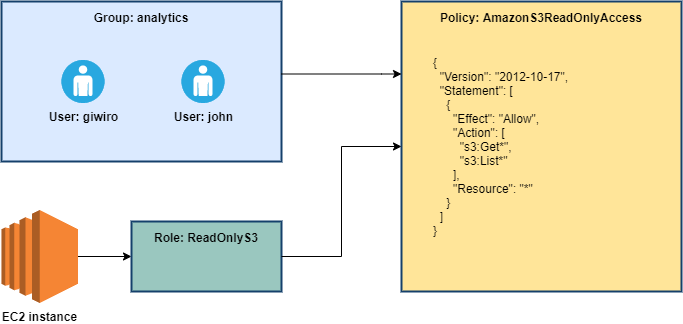
\includegraphics[scale=0.5]{iam/iam}
\centering
\end{figure}

\subsection{Access AWS}
\begin{itemize}
	\item{\textbf{Management Console:}} Web portal. Protected by password + MFA (Optional, but recomended)
	\item{\textbf{CLI:}} Command Line tool. Protected by access keys.
	\item{\textbf{SDK:}} Code library. Protected by access keys.
\end{itemize}

\subsection{IAM Security Tools}
\begin{itemize}
	\item{\textbf{IAM Credentials Report:}} Account level tool that lists all users and the status of their credentials.
\item{\textbf{IAM Access Advisor:}} User level tool. List of all permisions (policies) per service and when it was last accessed.
\end{itemize}

\subsection{IAM Share responsibility model}
\begin{itemize}
	\item{Management and monitoring of users, groups, roles and policies}
	\item{Enable MFA on all accounts}
	\item{Rotate all the keys often}
	\item{Analyze access patterns \& review permissions}
\end{itemize}
